% ============================================================================================
% BAB III ANALISIS MASALAH
% VERSI PERBAIKAN (04-Nov-2025)
% FIX:
% 1. Mengganti float '[t]' (top) menjadi '[H]' (Here) dari paket 'float'.
%    Ini "memaksa" tabel untuk tampil persis di tempat kode diletakkan
%    dan tidak mengambang ke bawah halaman.
%
% PENTING: Pastikan Anda sudah menambahkan \usepackage{float} di file .tex utama!
% ============================================================================================
\chapter{ANALISIS MASALAH}
\label{chap:analisis-masalah}

\section{Analisis Kondisi Saat Ini}
\label{sec:analisis-kondisi-saat-ini}

% --- Gambar Alur Proses As-Is ---
% FIX: Menggunakan [H] agar gambar tidak mengambang
\begin{figure}[H] 
	\centering
  \captionsetup{justification=centering}
    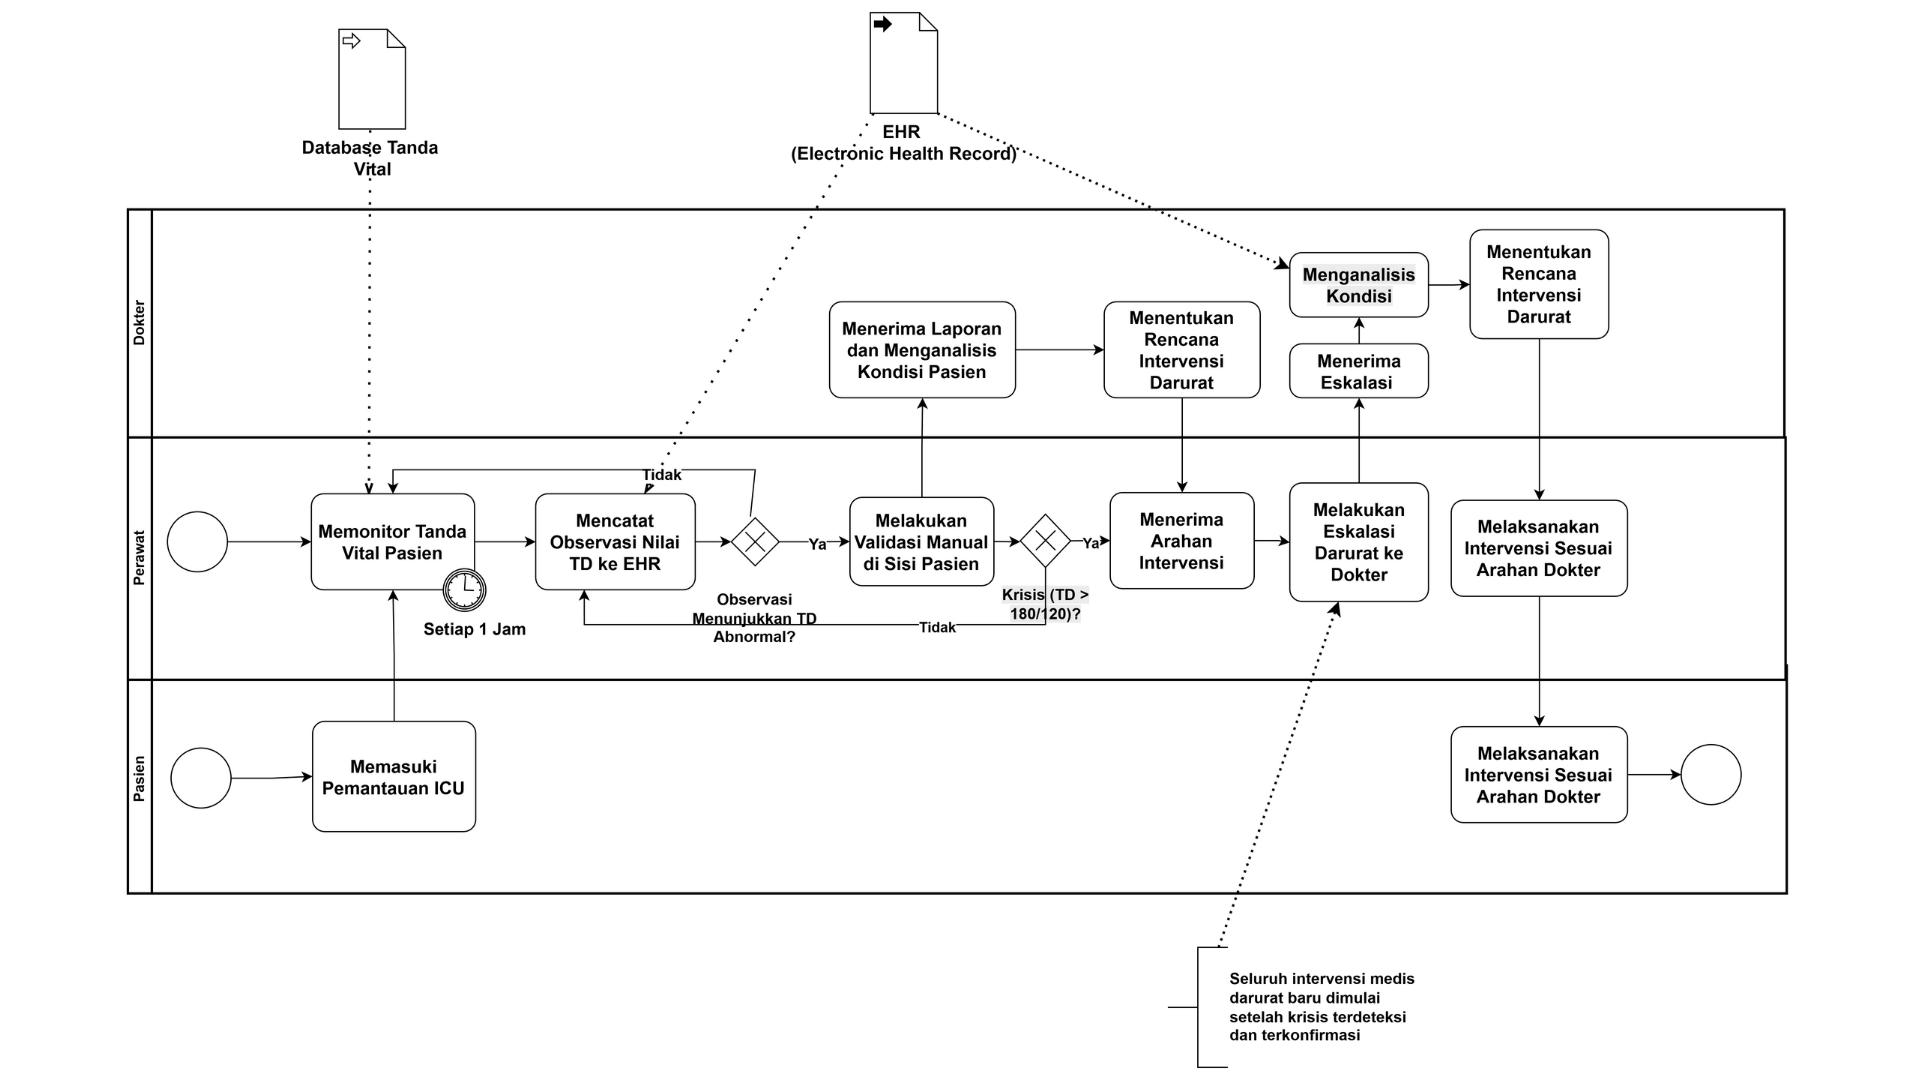
\includegraphics[width=0.9\textwidth]{image/gambar1.png} 
	\caption{Alur proses 'As-Is' manajemen klinis hipertensi}
	\label{gambar:alur-as-is}
\end{figure}

Proses manajemen klinis untuk pasien hipertensi saat ini beroperasi pada paradigma yang fundamentalnya bersifat reaktif. Alur kerja konvensional ini, seperti yang telah dimodelkan, bergantung pada intervensi yang baru dilakukan setelah diagnosis ditegakkan atau setelah terjadi fluktuasi tekanan darah (TD) yang signifikan. Kelemahan utama dari pendekatan ini adalah kegagalannya dalam mengantisipasi dan mencegah episode akut yang paling berbahaya, yaitu krisis hipertensi. Krisis hipertensi didefinisikan sebagai kondisi darurat medis di mana tekanan darah melonjak melebihi 180/120 mmHg. Kondisi ini secara langsung berpotensi menyebabkan kerusakan pada organ target, seperti stroke atau gagal jantung, sehingga menjadikannya tantangan serius bagi kesehatan masyarakat. Dengan demikian, alur kerja yang hanya menunggu terjadinya krisis adalah model yang secara inheren berisiko tinggi dan tidak memadai.

Urgensi untuk mengatasi masalah ini diperkuat oleh definisi klinis dari krisis hipertensi itu sendiri. Kondisi ini diklasifikasikan sebagai Hypertensive Emergency (Hipertensi Emergensi) ketika lonjakan TD yang parah (melebihi 180/120 mmHg) disertai dengan bukti adanya kerusakan organ target akut. Kerusakan ini dapat bermanifestasi secara cepat dan parah, meliputi perubahan status mental, infark miokard, gagal ginjal akut, atau diseksi aorta. Dalam paradigma "As-Is", alarm atau eskalasi ke dokter baru terjadi setelah kondisi yang mengancam jiwa ini dimulai, sehingga waktu penanganan yang krusial telah hilang. Identifikasi dan tatalaksana yang segera sangat penting untuk mencegah kerusakan organ permanen atau risiko kematian. Oleh karena itu, jelas bahwa sistem yang hanya "bereaksi" terhadap krisis yang sudah terjadi secara fundamental gagal dalam misi preventif.

Kebutuhan untuk bertransisi menuju manajemen proaktif kini menjadi mungkin berkat kemajuan dalam pengumpulan data dan machine learning. Ketersediaan dataset publik beresolusi tinggi, seperti MIMIC-IV, menyediakan rekaman data longitudinal yang rinci, termasuk data runtun waktu (time-series) dari tanda-tanda vital seperti nilai TD per jam. Data historis yang kaya ini merupakan prasyarat mutlak yang memungkinkan pelatihan model prediktif untuk memantau fluktuasi tekanan darah dari jam ke jam. Dengan memanfaatkan data ini, sebuah sistem dapat dikembangkan untuk memberikan peringatan dini. Tujuan utamanya adalah untuk memprediksi probabilitas terjadinya krisis hipertensi sebelum ambang batas 180/120 mmHg terlampaui, sehingga memungkinkan intervensi preventif.

Meskipun model machine learning (ML) seperti ensemble (Random Forest atau XGBoost) telah menunjukkan kinerja state-of-the-art dalam menangani data tabular kompleks, akurasi prediktif yang tinggi (high-fidelity) saja belum mencukupi untuk adopsi klinis. Hambatan utama dalam implementasi machine learning di lingkungan berisiko tinggi seperti perawatan kesehatan adalah sifat alaminya sebagai "kotak hitam" (black box). Masalah "black box" ini merujuk pada kurangnya transparansi dan interpretabilitas dari model-model kompleks. Meskipun model tersebut mampu menghasilkan prediksi (keluaran) yang sangat akurat, model tersebut tidak dapat memberikan justifikasi yang mudah dipahami manusia atas keputusan yang diambil. Opasitas ini menjadi masalah kritis di bidang kedokteran, di mana setiap rekomendasi otomatis harus dapat diverifikasi dan dipertanggungjawabkan.

Konsekuensi langsung dari masalah "black box" adalah terhambatnya kepercayaan dan akuntabilitas dari pengguna akhir, yaitu para klinisi. Seorang dokter tidak dapat memercayai atau menindaklanjuti sebuah peringatan "Risiko Krisis 85\%" jika sistem tidak dapat memberikan justifikasi yang masuk akal dan dapat ditindaklanjuti secara klinis. Kurangnya transparansi internal ini menciptakan keraguan, karena pengguna tidak dapat memverifikasi alasan di balik peringatan tersebut. Dalam domain di mana keputusan dapat berarti antara hidup dan mati, sistem yang tidak dapat dipertanggungjawabkan tidak akan pernah diadopsi sepenuhnya, tidak peduli seberapa akurat prediksinya. Kesenjangan kepercayaan ini adalah penghalang adopsi yang sama seriusnya dengan masalah paradigma reaktif itu sendiri.

Untuk menjembatani kesenjangan antara akurasi prediktif dan adopsi klinis, disiplin AI yang dapat dijelaskan (Explainable AI atau XAI) menjadi komponen yang krusial dan wajib ada. XAI menawarkan solusi untuk "membuka" kotak hitam dan memberikan transparansi yang dibutuhkan. Metode atribusi post-hoc yang kuat seperti SHAP (SHapley Additive exPlanations) secara khusus dirancang untuk mengatasi masalah ini. SHAP, yang didasarkan pada teori permainan kooperatif, mampu mengkalkulasi kontribusi spesifik dari setiap fitur (misalnya, 'usia', 'TD 3 jam terakhir') terhadap deviasi prediksi model dari nilai dasarnya. Metode ini secara efektif memberikan penjelasan yang terukur (baik secara global maupun lokal per individu) mengenai alasan di balik terbentuknya suatu prediksi risiko. Kemampuan untuk menyediakan rasionalisasi inilah yang akan mengubah model ML dari sekadar alat prediksi menjadi sistem pendukung keputusan yang dapat dipercaya.

% --- Subseksi Analisis Kesenjangan ditambahkan berdasarkan PDF baru ---
\subsection{Analisis Kesenjangan}
Dilakukan analisis kesenjangan berikut ini untuk memetakan secara terstruktur kondisi saat ini (As-Is) dengan kondisi ideal (To-Be) yang diharapkan dari solusi yang diusulkan. Pemetaan ini merangkum permasalahan inti yang dijabarkan dalam Tabel \ref{tbl:gap-analysis} ini.

% --- Tabel Analisis Kesenjangan ---
% FIX: Menggunakan [H] agar tabel tidak mengambang
\begin{table}[H] 
  \begin{tabularx}{\textwidth}{ | l | X | X | X |}
	\hline
	\textbf{Domain Masalah} & \textbf{Kondisi Saat ini (As-Is)} & \textbf{Kesenjangan (Gap)} & \textbf{Kondisi Ideal (To-Be)} \\
	\hline
	Manajemen Klinis (Proses) & 
    Paradigma intervensi bersifat reaktif. Tindakan medis darurat baru diambil setelah pasien mengalami krisis hipertensi (TD $> 180/120$ mmHg). & 
    Keterlambatan intervensi kritis dan risiko kerusakan organ target (stroke, gagal jantung) yang tidak terantisipasi karena kegagalan mendeteksi risiko lebih awal. & 
    Paradigma manajemen bersifat proaktif. Klinisi mendapatkan peringatan dini yang akurat untuk mengantisipasi risiko krisis sebelum terjadi. \\
	\hline
	Adopsi Teknologi & 
    Model machine learning (ML) yang akurat bersifat "black box". Klinisi tidak dapat memahami atau memverifikasi alasan di balik sebuah peringatan risiko. & 
    Hambatan adopsi dan kurangnya kepercayaan (trust) pada sistem cerdas. Sistem tidak akuntabel sehingga sulit diimplementasikan di lingkungan berisiko tinggi. & 
    Model ML bersifat transparan dan dapat dijelaskan. Sistem mampu memberikan justifikasi (via SHAP) untuk setiap prediksi risiko individu, sehingga membangun kepercayaan klinis. \\
	\hline
	Pemanfaatan Data (Sistem) & 
    Data runtun waktu (time-series) klinis beresolusi tinggi (dari MIMIC-IV) ada, namun belum dimanfaatkan secara optimal untuk prediksi antisipatif. & 
    Peluang yang terlewatkan. Data historis yang kaya hanya digunakan untuk analisis retrospektif, bukan untuk memprediksi dan mencegah outcome buruk secara proaktif. & 
    Data time-series diproses melalui alur kerja (pipeline) rekayasa fitur untuk melatih model ML yang mampu mengubah data historis menjadi peringatan dini yang dapat ditindaklanjuti. \\
	\hline
  \end{tabularx}
  \caption{Analisis Kesenjangan (Gap Analysis)}
  \label{tbl:gap-analysis}
\end{table}

Di sini diketahui bahwa masalah yang dihadapi bersifat multifaset, mencakup aspek proses klinis (paradigma reaktif) dan aspek teknologi (masalah "black box"). Kesenjangan ini menunjukkan kebutuhan mendesak akan sebuah solusi cerdas yang tidak hanya menyajikan prediksi outcome, tetapi juga mampu menyajikan rasionalisasi dari prediksi tersebut untuk membangun kepercayaan. Untuk dapat merancang solusi yang efektif dalam menutup kesenjangan ini, langkah selanjutnya adalah menerjemahkan kebutuhan tersebut ke dalam spesifikasi fungsional dan non-fungsional yang terukur.

\section{Analisis Kebutuhan}
Berdasarkan analisis kesenjangan yang telah dipaparkan sebelumnya, langkah selanjutnya adalah menerjemahkan kebutuhan solusi menjadi serangkaian spesifikasi yang terukur. Tahap ini krusial untuk memastikan bahwa sistem yang akan dikembangkan, yaitu purwarupa "Digital Twin Sederhana", secara langsung menjawab dua masalah fundamental yang telah diidentifikasi. Spesifikasi ini akan dibagi menjadi tiga kategori utama: identifikasi masalah spesifik dari kacamata pengguna, kebutuhan fungsional (apa yang harus dilakukan sistem), dan kebutuhan non-fungsional (kriteria kualitas sistem). Proses pendefinisian kebutuhan ini akan menjadi cetak biru (blueprint) yang memandu seluruh alur kerja penelitian, mulai dari akuisisi data hingga perancangan prototipe.

\subsection{Identifikasi Masalah Pengguna}
Pengguna utama dari sistem "To-Be" yang diusulkan adalah Klinisi di lingkungan perawatan intensif, yang mencakup Dokter (sebagai pengambil keputusan) dan Perawat (sebagai pelaksana monitor dan intervensi). Berdasarkan analisis kondisi "As-Is" (3.1), kedua pengguna ini menghadapi dua masalah spesifik yang saling terkait. Masalah pertama adalah beban kognitif dan risiko keterlambatan intervensi akibat paradigma reaktif. Perawat ICU dihadapkan pada beban kerja pemantauan manual yang tinggi, di mana mereka harus mengamati tanda vital pasien secara periodik (misal, per jam). Masalahnya, krisis hipertensi dapat berkembang cepat di antara interval pengecekan, sehingga memunculkan risiko kesalahan manusiawi (human error) atau deteksi yang terlambat. Bagi Dokter, masalahnya adalah mereka baru menerima eskalasi darurat setelah pasien berada dalam kondisi krisis, sehingga kehilangan waktu emas untuk melakukan pencegahan.

Masalah kedua adalah ketidakpercayaan dan keraguan adopsi akibat sistem "kotak hitam". Ketika sebuah solusi teknologi (seperti model ML) ditawarkan untuk mengatasi masalah pertama, pengguna klinis dihadapkan pada masalah baru: ketidakmampuan untuk memvalidasi atau memahami mengapa sebuah peringatan risiko muncul. Bagi Dokter, masalah ini sangat fundamental karena mereka tidak dapat menindaklanjuti (misalnya, memberikan obat preventif) sebuah peringatan yang tidak dapat dijelaskan. Hal ini menciptakan masalah turunan berupa "keraguan dalam pengambilan keputusan" (hesitancy to act) dan masalah "akuntabilitas", di mana klinisi tidak dapat bertanggung jawab atas keputusan yang didasarkan pada alat yang buram (opaque). Oleh karena itu, masalah pengguna yang teridentifikasi bukan hanya "butuh prediksi", tetapi "butuh prediksi yang dapat dipercaya dan dijelaskan.".

\subsection{Kebutuhan Fungsional}
Kebutuhan fungsional (Functional Requirements) adalah pernyataan spesifik mengenai fungsionalitas atau layanan inti yang harus disediakan sistem untuk memecahkan masalah pengguna yang teridentifikasi di 3.2.1. Kebutuhan ini diturunkan secara langsung dari alur kerja penelitian yang diuraikan dalam Bab 1.5 dan bertujuan untuk menutup kesenjangan teknis yang ada. Setiap fungsi harus dapat diimplementasikan dan diuji untuk memvalidasi bahwa sistem mampu mengeksekusi tugas-tugas yang diperlukan untuk mencapai tujuan proaktif dan dapat dijelaskan. Fungsi-fungsi ini mencakup seluruh siklus hidup data, mulai dari pemrosesan data mentah, transformasi fitur, pemodelan, hingga visualisasi hasil akhir. Kebutuhan fungsional dijabarkan sebagai berikut:

% --- Tabel Kebutuhan Fungsional ---
% FIX: Menggunakan [H] agar tabel tidak mengambang
\begin{table}[H] 
  \begin{tabularx}{\textwidth}{ | l | p{4cm} | X |}
	\hline
	\textbf{ID} & \textbf{Kebutuhan Fungsional} & \textbf{Deskripsi} \\
	\hline
	F-01 & Manajemen \& Ekstraksi Data & 
    Sistem terbukti mampu memuat file .csv dari dataset MIMIC-IV Demo (100 pasien). Sistem harus mampu memvalidasi dan mengekstrak kohort pasien krisis (27 pasien unik yang teridentifikasi). \\
	\hline
	F-02 & Rekayasa Fitur (Feature Engineering) & 
    Sistem mampu menghasilkan satu tabel fitur (X) statis dan satu tabel target (Y) biner ($1=\text{Krisis}, 0=\text{Aman}$). Tabel fitur (X) wajib mencakup fitur statis (usia, gender) dan fitur agregat/tren (misal: rata-rata, slope TD). \\
	\hline
	F-03 & Pemodelan Prediktif & 
    \\
	\hline
	F-04 & Implementasi Interpretabilitas (XAI) & 
    Sistem mampu menghasilkan visualisasi SHAP Summary Plot untuk penjelasan global. Sistem juga wajib mampu menghasilkan visualisasi SHAP Force Plot atau Waterfall Plot untuk setiap prediksi individu (penjelasan lokal). \\
	\hline
	F-05 & Visualisasi Prototipe CDSS (Dashboard) & 
    Sistem (dibangun dengan Streamlit) mampu menampilkan secara bersamaan: (1) Skor prediksi risiko (dari F-3) dan (2) Visualisasi penjelasan SHAP (dari F-4) dalam satu antarmuka dashboard interaktif. \\
	\hline
  \end{tabularx}
  \caption{Kebutuhan Fungsional}
  \label{tbl:kebutuhan-fungsional}
\end{table}

\subsection{Kebutuhan Nonfungsional}
Kebutuhan non-fungsional (Non-Functional Requirements) mendefinisikan kriteria kualitas, batasan operasional, dan atribut sistem yang tidak terkait langsung dengan fungsi spesifik. Dalam konteks penelitian medis ini, kebutuhan non-fungsional sama pentingnya dengan kebutuhan fungsional karena menentukan validitas, kepercayaan, dan reliabilitas dari solusi yang diusulkan. Kebutuhan ini menetapkan standar "seberapa baik" sistem harus bekerja, bukan hanya "apa" yang harus dilakukannya. Berikut adalah kebutuhan non-fungsional utama untuk sistem ini:

% --- Tabel Kebutuhan Nonfungsional ---
% FIX: Menggunakan [H] agar tabel tidak mengambang
\begin{table}[H] 
  \begin{tabularx}{\textwidth}{ | l | p{4cm} | X |}
	\hline
	\textbf{ID} & \textbf{Kebutuhan Non-Fungsional} & \textbf{Deskripsi (Kriteria Kualitas yang Terukur)} \\
	\hline
	NFR-01 & Transparansi & 
    Sistem harus 100\% dapat dijelaskan. Setiap prediksi risiko yang dihasilkan (F-3) wajib disertai dengan visualisasi penjelasan SHAP (F-4) yang menunjukkan kontribusi fitur-fitur pendorong risiko. \\
	\hline
	NFR-02 & Kinerja Prediktif & 
    Kinerja model pada test set wajib dievaluasi menggunakan metrik utama AUC-ROC. Kinerja juga harus dilaporkan menggunakan Precision dan Recall, dengan penekanan analisis pada minimalisasi False Negative (pasien krisis yang diprediksi aman). \\
	\hline
	NFR-03 & Kebergunaan (Usability) & 
    Visualisasi SHAP (F-4) pada dashboard (F-5) harus dapat dipahami secara intuitif oleh pengguna non-teknis (klinisi). Faktor pendorong risiko (fitur) harus disajikan dengan jelas, tanpa jargon ilmu data yang kompleks. \\
	\hline
	NFR-04 & Lingkup Prototipe & 
    Sistem beroperasi sebagai purwarupa dalam lingkungan simulasi (offline). Output sistem (skor risiko \& SHAP) berfungsi sebagai pendukung keputusan, bukan diagnosis medis otomatis. \\
	\hline
  \end{tabularx}
  \caption{Kebutuhan Nonfungsional}
  \label{tbl:kebutuhan-nonfungsional}
\end{table}

\section{Analisis Pemilihan Solusi}
Dalam merancang sistem "Digital Twin Sederhana" untuk prediksi krisis hipertensi, diperlukan analisis terhadap permasalahan dan potensi peluang untuk merumuskan solusi yang paling tepat. Sub-bab ini menyajikan pemetaan masalah dan peluang yang diidentifikasi dari sub-bab 3.1. Setelah itu, akan dipaparkan perbandingan alternatif solusi teknologi yang relevan, yang kemudian akan dievaluasi menggunakan kerangka kerja formal untuk menentukan solusi terpilih.

\subsection{Alternatif Solusi}
Permasalahan yang muncul dalam lingkup penelitian tugas akhir ini perlu dikaji satu per satu agar penulis dapat merumuskan solusi yang relevan. Identifikasi masalah utama yang telah ditemukan (dari sub-bab 3.1) dijabarkan pada Tabel \ref{tbl:pemetaan-masalah}.

% --- Tabel Pemetaan Masalah ---
% FIX: Menggunakan [H] agar tabel tidak mengambang
\begin{table}[H]
  \begin{tabularx}{\textwidth}{ | l | X | X |}
	\hline
	\textbf{ID} & \textbf{Masalah} & \textbf{Dampak} \\
	\hline
	M01 & Paradigma klinis reaktif; intervensi baru dilakukan setelah krisis hipertensi terjadi. & Risiko kerusakan organ target (stroke, gagal jantung) yang tinggi akibat keterlambatan intervensi preventif. \\
	\hline
	M02 & Model machine learning (ML) bersifat "black box" dan tidak transparan bagi klinisi. & Hambatan adopsi dan kurangnya kepercayaan (trust). Klinisi tidak dapat memvalidasi atau menindaklanjuti peringatan yang tidak dapat dijelaskan. \\
	\hline
	M03 & Data klinis (vital sign) bersifat runtun waktu (time-series) dan kompleks. & Sulit melakukan pemrosesan otomatis oleh model ML tabular (seperti XGBoost/RF) tanpa transformasi data terlebih dahulu. \\
	\hline
  \end{tabularx}
  \caption{Pemetaan Masalah}
  \label{tbl:pemetaan-masalah}
\end{table}

Uraian permasalahan di atas menunjukkan bahwa didapati kebutuhan akan sistem yang dapat beralih ke paradigma proaktif dan menyajikan informasi risiko yang akurat serta dapat dipercaya. Di sisi lain, proyek yang berakar dari permasalahan ini memiliki potensi besar untuk dikembangkan, yang pemetaan peluangnya dijabarkan pada Tabel \ref{tbl:pemetaan-peluang}.

% --- Tabel Pemetaan Peluang ---
% FIX: Menggunakan [H] agar tabel tidak mengambang
\begin{table}[H]
  \begin{tabularx}{\textwidth}{ | l | l | X |}
	\hline
	\textbf{ID} & \textbf{Pemetaan Masalah} & \textbf{Peluang} \\
	\hline
	P01 & M01, M02 & Memungkinkan untuk perancangan CDSS proaktif yang mengintegrasikan modul prediksi risiko (mengatasi M01) dan modul XAI (mengatasi M02). \\
	\hline
	P02 & M03 & Ketersediaan dataset MIMIC-IV Demo (Data 1/Notulensi) yang dapat digunakan untuk melatih model machine learning. \\
	\hline
	P03 & M03 & Teknik Rekayasa Fitur (Feature Engineering) (F-2) memungkinkan ekstraksi fitur tabular yang relevan dari data runtun waktu yang kompleks. \\
	\hline
	P04 & M01 & Algoritma machine learning (seperti XGBoost) dari studi literatur terbukti state-of-the-art untuk data tabular klinis (mendukung F-3). \\
	\hline
	P05 & M02 & Algoritma XAI (SHAP) dari studi literatur (Data 1/Bab 2) dapat digunakan untuk memberikan transparansi dan membangun kepercayaan (mendukung F-4). \\
	\hline
  \end{tabularx}
  \caption{Pemetaan Peluang (Proyek Hipertensi)}
  \label{tbl:pemetaan-peluang}
\end{table}

Penulis mengevaluasi berbagai pendekatan teknis yang dapat diadopsi dalam membangun sistem prediksi krisis hipertensi, yang dijabarkan dalam Tabel \ref{tbl:alternatif-solusi} di bawah ini.

% --- Tabel Alternatif Solusi ---
% FIX: Menggunakan [H] agar tabel tidak mengambang
\begin{table}[H]
  \begin{tabularx}{\textwidth}{ | l | p{3.5cm} | X | X |}
	\hline
	\textbf{No.} & \textbf{Solusi} & \textbf{Kelebihan (Pros)} & \textbf{Kekurangan (Cons)} \\
	\hline
	1. & Model Statistik Dapat Diinterpretasi (cth: Regresi Logistik) & 
    Sangat Transparan: Model bersifat "white box" dan inheren dapat dijelaskan. \newline Sederhana: Komputasi ringan dan mudah diimplementasikan. & 
    Kinerja Terbatas: Cenderung memiliki kinerja prediktif yang lebih rendah pada data medis yang non-linear dan kompleks. \\
	\hline
	2. & Model Deep Learning (cth: LSTM/RNN) & 
    Kinerja Sangat Tinggi: Sangat baik dalam menangkap pola data runtun waktu mentah. & 
    "Black Box" Ekstrem: Sangat sulit diinterpretasikan (gagal memenuhi NF-1). \newline Kompleksitas Tinggi: Membutuhkan komputasi besar dan implementasi yang rumit. \\
	\hline
	3. & Model Ensemble + XAI (cth: XGBoost + SHAP) & 
    Kinerja Tinggi: Performa state-of-the-art pada data tabular (hasil F-2). \newline Transparan (via XAI): Memenuhi NF-1 dengan menyediakan penjelasan post-hoc (SHAP). \newline Seimbang: Keseimbangan terbaik antara Kinerja (NF-2) dan Transparansi (NF-1). & 
    Memerlukan Rekayasa Fitur (Feature Engineering): Kinerja sangat bergantung pada kualitas fitur yang diekstraksi (F-2). \\
	\hline
  \end{tabularx}
  \caption{Alternatif Solusi}
  \label{tbl:alternatif-solusi}
\end{table}

\subsection{Analisis Penentuan Solusi}
Dalam menentukan pendekatan teknis dalam merancang sistem ini, dilakukan evaluasi menggunakan metode Weighted Scoring Matrix (WSM). WSM adalah sebuah teknik yang mengombinasikan ukuran kualitatif dan kuantitatif dengan cara memberikan skor pada setiap alternatif solusi terhadap serangkaian kriteria yang relevan. Metode ini dipilih karena dianggap tidak terlalu kompleks, fleksibel, dan bobotnya dapat disesuaikan berdasarkan aspek sesuai topik model yang akan dikembangkan. Masing-masing parameter penghitungan bobot diperoleh dari kebutuhan non-fungsional (Tabel \ref{tbl:kebutuhan-nonfungsional}) yang telah dijabarkan sebelumnya. Bobot ditentukan berdasarkan prioritas penelitian, di mana Kinerja Prediktif (NF-2) dan Transparansi (NF-1) dianggap sebagai prioritas utama. 
Setiap alternatif solusi diberikan nilai antara 1 hingga 5 ($1 = \text{sangat buruk}, 5 = \text{sangat baik}$). Skor akhir diperoleh dari perkalian nilai dengan bobot masing-masing parameter yang dijabarkan pada Tabel \ref{tbl:wsm}.

% --- Tabel WSM ---
% FIX: Menggunakan [H] agar tabel tidak mengambang
\begin{table}[H]
  \centering 
  \begin{tabular}{ | l | c | >{\centering\arraybackslash}p{2.5cm} | >{\centering\arraybackslash}p{2.5cm} | >{\centering\arraybackslash}p{3cm} |}
	\hline
	\textbf{Parameter} & \textbf{Bobot} & \textbf{1. Regresi Logistik} & \textbf{2. Deep Learning (LSTM)} & \textbf{3. Ensemble + SHAP} \\
    & & Skor (1-5) & Skor (1-5) & Skor (1-5) \\
	\hline
	Kinerja Prediktif (NF-2) & 0,45 & 2 & 5 & 4 \\
	Transparansi (NF-1) & 0,45 & 5 & 1 & 4 \\
	Kompleksitas Implementasi & 0,10 & 5 & 1 & 3 \\
	\hline
	\textbf{Total Skor} & \textbf{1,00} & \textbf{3.65} & \textbf{2.80} & \textbf{3.90} \\
	\hline
  \end{tabular}
  \caption{Pemilihan Solusi dengan Weighted Scoring Model (WSM)}
  \label{tbl:wsm}
\end{table}

% --- Subseksi Solusi Terpilih ---
\subsection{Solusi Terpilih}
Berdasarkan perhitungan skor total pada Tabel \ref{tbl:wsm}, solusi yang akan diadopsi dalam konteks penelitian tugas akhir ini adalah \textbf{Alternatif 3: Model Ensemble + XAI (XGBoost + SHAP)} dengan skor akhir tertinggi yaitu 3,90. Model ini dianggap mampu menangani data tabular hasil rekayasa fitur (F-2) dengan keandalan tinggi, sekaligus memenuhi kebutuhan non-fungsional krusial NF-1 (Transparansi). Solusi ini dipilih karena memberikan keseimbangan terbaik antara kinerja prediktif dan interpretabilitas, yang merupakan dua pilar utama untuk mengatasi masalah yang telah diidentifikasi.